\section{Auswertung}
\label{sec:Auswertung}

\begin{figure}[H]
  \centering
  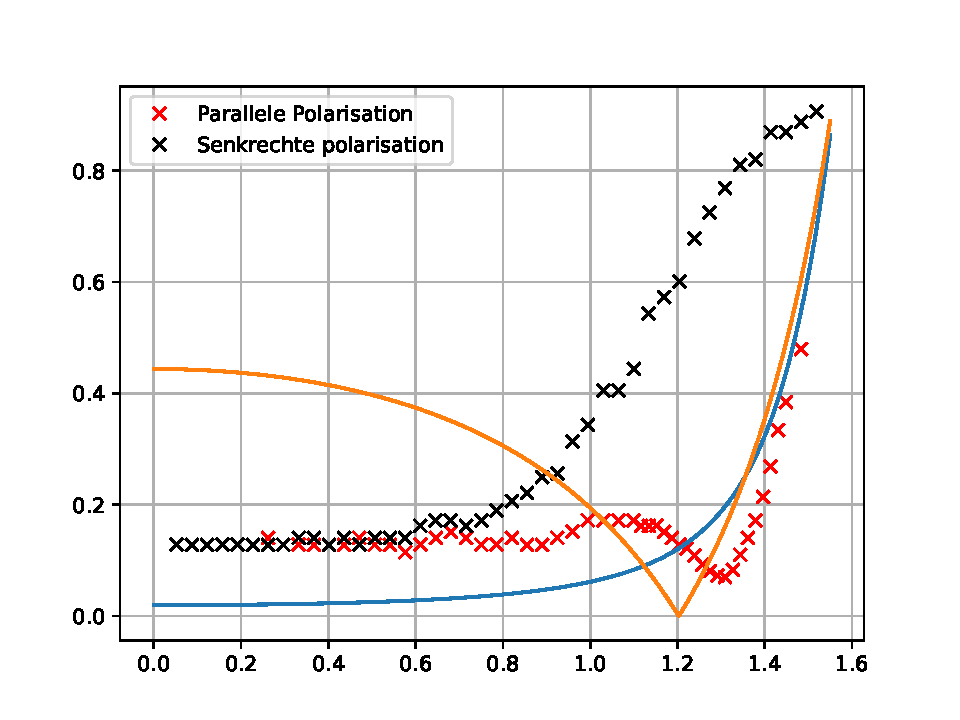
\includegraphics{plot.pdf}
  \caption{Lineare Ausgleichkurve}
  \label{fig:plot}
\end{figure}

\begin{table}
  \centering
  \caption{Kraftwerte Der Federauslenkung.}
  \label{tab:tabelle}
  \sisetup{table-format=1.1, per-mode=reciprocal}
  \begin{tblr}{
      colspec = {S[table-format=1.0] S[table-format=1.2] S},
      row{1} = {guard, mode=math},
      %vline{4} = {2}{-}{text=\clap{$\pm$}},
    }
    \toprule
    \Delta x &  \symbf{F}(cm) & \symbf{D} & \\
    \midrule
    2 & 0.06 & 0.03 &  \\
    4 & 0.12 & 0.03 &  \\
    6 & 0.18 & 0.03 &  \\
    8 & 0.24 & 0.03 &  \\
    10 & 0.29 & 0.029 &  \\
    12 & 0.36 & 0.03 &  \\
    14 & 0.41 & 0.0292 &  \\
    16 & 0.47 & 0.0293 &  \\
    18 & 0.53 & 0.0294 &  \\
    20 & 0.59 & 0.0295 &  \\
    \bottomrule
  \end{tblr}
\end{table}







Mit den Messwerten aus der Tabelle kann man nun mit der 
Formel \autoref{eq:example} und dem Mittelwert $0.058\symbf{N}/2 cm$ die Ferderkonstante $\symbf{D}$
zu $0.058\symbf{N}/2 cm = 0.029 \symbf{N}/cm$ bestimmen.

%Siehe \autoref{fig:plot} und \autoref{tab:tabelle}!
